
\documentclass[preprint,12pt]{elsarticle}
\usepackage[margin=1in]{geometry}

\usepackage{siunitx}
\usepackage[font=footnotesize, justification = centering]{caption}
\usepackage[font=footnotesize]{subcaption}
\usepackage{amsmath}
\usepackage[ruled,vlined]{algorithm2e} %for writing pseudocodes
\usepackage{graphicx}

\journal{Journal of Computer Networks and Applications}

\begin{document}
	\begin{frontmatter}
		\title{Static and Dynamic Controller Assignment Algorithms for Software-Defined Networks}
		
		\author{Talha Ibn Aziz}
		\address{Department of Computer Science and Engineering, Islamic University of Technology, Dhaka, Bangladesh, Email: talhaibnaziz@iut-dhaka.edu}
		
		\begin{abstract}
			Software-Defined Networks (SDNs) are replacing traditional networks in several data centers by virtue of its programmability and efficient use of resources. Increasing network sizes demand multiple decision taking entities to monitor and operate the ever-changing networks. The resultant NP-Hard problem - also known as \textit{the Controller Placement Problem (CPP)} is a center-stage for intensive research. Many approaches over the years address various parameters of the controller placement paradigm, like flow-setup latencies, load balancing, reliability and resilience. However, very few provide an efficient algorithm which addresses multiple parameters in polynomial-time complexity. I propose a novel controller assignment method which minimizes overall flow-setup latency, route-synchronization latency and controller response times simultaneously, by dividing the network into several clusters, placing controllers and assigning switches dynamically. Simulation results show that my proposed mechanism outperforms existing state-of-the-art algorithms in terms of overall network setup latencies.
		\end{abstract}
		\begin{keyword}
			SDN \sep CPP \sep controllers \sep flow-setup \sep latency
		\end{keyword}
		
	\end{frontmatter}

	\section{Introduction}
	Software Defined Networks (SDNs) simplify network management by decoupling the traditional protocol stack into data and control planes, which consist of switches and controllers, respectively. The controllers replace the switches as the decision taking entities of the SDNs and the switches only retain their data-forwarding capabilities, which simplifies switch designs and configurations. Due to scalability and reliability issues \cite{scalability2013dixit, scalability2013yeganeh} paired with the formation of bottle-necks in moderate-sized networks, the initial design of a single controller \cite{greene2009tr10} is replaced by a multiple-controller architecture. The resultant problem is well-known as the NP-Hard Controller Placement Problem (CPP) which deals with placing an optimal number of controllers to improve network throughput \cite{cppsurvey2017, cppsurvey2018, sdnsurvey2017}. The multiple constraints that need satisfying include minimizing network latencies, deployment costs, energy consumption and maximizing reliability and resilience. Researches in recent years propose several approximations which deal with one or more of these constraints.
	
	Initial experiments study the effects of different latencies on overall network throughput through exhaustive controller deployment \cite{cpp2012heller}. Eventually, other constraints like reliability \cite{hu2013reliability} and resilience \cite{zhang2011resilience} are addressed. Some approaches balance controller loads when placing them \cite{yao2014capacitated}, while others propose a more dynamic approach \cite{yao2015controller}. Several models have been developed to reduce deployment costs \cite{sallahi2015optimal} and controller response times \cite{wang2016dynamic}. Some researches also address multiple constraints by providing trade-off decisions to network operators, between certain performance parameters. Seeing that most of the afore-mentioned methods provide exhaustive solutions to the CPP, a few researches propose efficient polynomial-time algorithms to cluster the network \cite{dbcp2017} and balance load through both static \cite{dbcp2017} and dynamic assignments of controllers \cite{filali2018sdn}. However, they perform optimization of a specific parameter, instead of providing a complete system. To the best of my knowledge, there is no such method which clusters the network, places the controllers and assigns them dynamically to minimize overall latency and load imbalance in polynomial time complexity. In this paper, I propose a novel controller assignment method which minimizes the following:
	\begin{enumerate}
		\item \textbf{Flow-setup latency and Route synchronization latency:} When a new flow arrives at a switch, the flow-setup process is initiated through which the corresponding controller calculates a new path and notifies the concerned switches. Similarly, when there is a change in the network, the concerned controllers and switches have to be notified. The delay produced by these processes are called the flow-setup latency and the route-synchronization latency.
		\item \textbf{Controller response time and Load imbalance:} Due to the influx of numerous new flows, several query packets from multiple switches impose on the controllers. A great volume of processing is required to facilitate smooth operation of the network, which is called the \textit{load of a controller}. An imbalanced distribution of load can lead to an exponential increase of controller response times.
	\end{enumerate}
	The processing delays of SDN switches are significantly reduced compared to traditional networks and propagation latencies are also negligible. Therefore, overall network latency depends on transmission and queuing latencies of packets \cite{forouzan2006data}. My proposed method aims to divide the network into $k$ balanced clusters and place controllers to reduce transmission latency. Furthermore, the controller response time is improved through dynamic load balancing, which reduces queuing latency. Simulation results suggest that my proposed method outperforms the state-of-the-art algorithms in terms of overall network latency and load balancing.
	
	The remainder of my paper contains the system model and problem formulation in Section \ref{sysMod}, the detailed proposed mechanism in Section \ref{proposal}, the simulations and experimental analysis in Section \ref{simulations}, and the conclusion in Section \ref{conclusion}.
	
	\section{System Model and Assumptions} \label{sysMod}
	The network is represented as a bi-directional graph $G=(S,L)$, where, $S$ represents the set of switches (or nodes) and $L$ represents the set of links (or edges) between the switches. The edge weights represent link bandwidth i.e., the distance between two switches which is expressed as the transmission latency of sending a standard data packet from source to destination. The graph $G$ is clustered into multiple sub-network (or clusters) such that, each sub-network is a disjoint set of switches. All the switches must fall into some sub-network containing a single controller and no switch can have more than one controller. Therefore, I assume that the network is partitioned into $k$ sub-networks and the network is managed by a total of $k$ controllers. For simplicity I make the following assumptions:
	\begin{enumerate}
		\item The propagation delay of all control packets and the processing delay of all switch-to-controller control packets are negligible.
		\item A controller can only be placed on a switch location and all switch locations are called potential \textit{controller positions}.
		\item All the controllers have identical processing capacity.
	\end{enumerate}
	Following these assumptions, my goal is to minimize the flow-setup latency and controller processing time, which are measured in milliseconds. According to Little's law, the average response time of a controller is $\frac{1}{(Power_{C_i} - Load_{C_i})}$ \cite{wang2016dynamic}, where $Power_{C_i}$ is the maximum processing power and $Load_{C_i}$ is the \textit{load} of any controller $C_i$ of the network $S$. Therefore, I balance the $load$ of a controller to reduce average controller response time.
	
	\section{Proposed Method} \label{proposal}
	
	My proposed method consists of three algorithms - Latency Based Clustering (LBC), Controller Selection Algorithm (CSA) and Best-first-search Load Balancing (BLB). LBC clusters the network into a given number of sub-networks ($k$) and CSA places a controller in each sub-network, resulting in a static controller-switch assignment. BLB is a dynamic load balancing algorithm which periodically reassigns switches to avoid over-burdening a controller. The above mentioned algorithms are explained in detail in sections \ref{lbc}, \ref{csa} and \ref{blb}, respectively.
	
	\subsection{Latency Based Clustering (LBC)} \label{lbc}
	
	%Explain what our previous work did and what are its shortcomings
	My previous work Degree-based Balanced Clustering (DBC) \cite{aziz2019degree} selects the nodes with the highest degrees in an unweighted network as cluster heads to facilitate better communication. Ensuring that the cluster heads are a minimum distance ($T_d$) apart from each other, DBC places controllers based on inter-controller and intra-controller distances. However, the controllers are rarely in the same positions as the cluster heads, invalidating the degree-based cluster head selection. I propose a novel clustering algorithm LBC, which selects cluster-centers instead of cluster-heads. These cluster-centers are the foundations of the clusters as they ensure that the clusters are evenly distributed throughout the network and not centralized at a certain region.
	
	Assuming the network is small enough to be managed by a single controller, it should be placed at the center of the network, as the controller communicates frequently with the switches. The center of a graph is the node with the minimum distance from all other nodes \cite{wilson1979introduction}, and can be determined by minimizing the average or maximum distance from every other node:
	
	\begin{equation} \label{eqn:avgDis}
	center_{avg} = \min_{s\in S}\bigg(\frac{\sum_{d\in S}^{d\ne s}dis(s,d)}{|S|-1}\bigg)
	\end{equation}
	\begin{equation} \label{eqn:maxDis}
	center_{max} = \min_{s\in S}\bigg(max_{d\in S}\big(dis(s,d)\big)\bigg)
	\end{equation}
	
	\begin{figure}
		\centering
		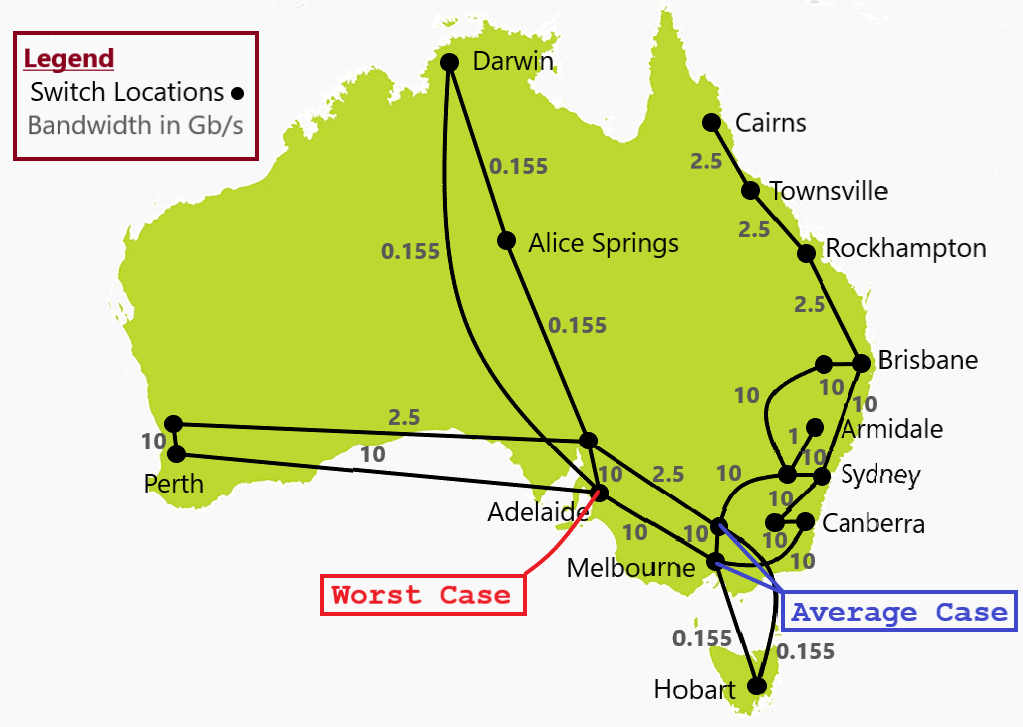
\includegraphics[width=0.85\linewidth]{Images/Aarnet.png}
		\caption{Existing network of Australia (AARNET \cite{knight2011internet}) showing the centers of the network.}
		\label{fig:aarnetcc}
	\end{figure}
	
	here, $center_{avg}$ and $center_{max}$ are the centers of the network $S$, being the nearest to any other node in terms of average and maximum distances, respectively. The shortest path distance from $s$ to $d$ is denoted by $dis(s,d)$. The maximum distance or worst case latency (Equation \ref{eqn:maxDis}), when determines the center of the network, can vary greatly in the presence of distant and isolated nodes (Figure \ref{fig:aarnetcc}). Conversely, the average case latency (Equation \ref{eqn:avgDis}) is unaffected by outliers. Therefore, I select the node with the minimum average distance as the center ($center_{avg}$) of the network.
	
	For larger networks however, when placing multiple controllers, multiple sub-networks must be formed which makes the center selection process troublesome. To ensure equal division of the network, the cluster-centers must be equidistant from each other and the clusters must expand from the centers. This selection of centers in a network is a classical NP-hard problem of computer science - \textit{The vertex k-center problem} \cite{kariv1979algorithmic}, which has many optimal approximations. My algorithm LBC (Algorithm \ref{algo:lbc}) utilizes the latencies between switches to divide the network optimally while ensuring that each cluster contains potential controller positions.
	
	\begin{algorithm}
		\SetAlgoLined
		\KwResult{Set of Cluster-Centers, $CC$ }
		$dis := all~possible~node~pair~shortest~distances$\;
		for all $s\in S$, $\overline{Dis}_s := \frac{\sum_{s,d \in S}^{d \ne s}dis(s,d)}{|S|-1}$\;
		$CC := \emptyset$, $k :=$ required number of controllers\;
		\While{$|CC| < k$}{
			$CC := CC \cup \{s_{cc}\}$ for all $s_{cc}\in S$, where $\overline{Dis}_{s_{cc}} \le \overline{Dis}_{t\in S}$\; 
			Create a new cluster $S_i$ which consists of $s_{cc}$ and $\big(\frac{|S|}{k}-1\big)$ nearest neighbors of $s_{cc}$ in terms of hop distance\;
			\ForEach{switch $s_i \in S_i$}{
				Subtract $\frac{dis(s_i, s)}{|S|-1}$ from $\overline{Dis}_s$ for all ${s \in S-S_i}$
			}
			$S = S - S_i$
		}
		\caption{Latency Based Clustering (LBC)} \label{algo:lbc}
	\end{algorithm}
	Ideally, a network $S$ containing $|S|$ switches and $k$ controllers, should have $\frac{|S|}{k}$ switches in each cluster. Therefore, every two cluster-center must have enough distance in between them to accommodate at least $\frac{|S|}{k}$ switches, which can be considered the \textit{ideal cluster-size}. The average distance of a node from all other nodes in the network increases gradually from the center towards the periphery. Accordingly, the node $s_{cc}$ with the minimum average distance $\overline{Dis_{s_{cc}}}$, is selected as the first cluster-center and the cluster is expanded hop by hop until the cluster-size reaches $\frac{|S|}{k}$ nodes. Consequently, the nodes of the cluster are removed from the network $S$ and their distances are subtracted from the average distances of the remaining nodes. This process is continued until $k$ clusters have been formed.
	
	\subsection{Controller Selection Algorithm (CSA)} \label{csa}
	
	The algorithm LBC provides a list of cluster-centers which are the starting points for each sub-network. The Controller Selection Algorithm (CSA) creates clusters once more from these cluster-centers to avoid formation of overlapping clusters or isolated cluster-centers, and then selects a controller position for each cluster. The nodes are included in the clusters of the nearest clusters-centers in terms of shortest path distance $dis(i,j)_{i,j \in S}$, which ends the cluster formation process and initiates the controller selection process (Algorithm \ref{algo:csa}). It is to be noted that the shortest path distance is not in terms of hop-counts.
	
	
	\begin{algorithm}
		\SetAlgoLined
		\KwResult{Set of Controllers, $C$ }
		$dis := all~possible~node~pair~shortest~distances$\;
		$CC_{i=1}^k :=$ \textbf{LBC}~Cluster~Centers\;
		$\phi_{s\in S}(s) :=$ intra-cluster latency of $s$\;
		$\sigma_{s\in S}(s) :=$ inter-cluster latency of $s$\;
		Form clusters $S_{i=1}^k$, each containing a cluster-center $CC_i$ and all its nearest nodes\;
		\ForEach{node $s \in S$}{
			$\phi(s)_{s\in S_i}=\frac{\sum_{t\in S_i} dis(s,t)}{|S_i|}$\;
			$\sigma(s)_{s\in S_i}=\frac{\sum_{t\in (S-S_i)} dis(s,t)}{|S-S_i|}$\;
		}
		\ForEach{node $s$ in cluster $S_i \subset S$}{
			$s_c:=\min\bigg(\big( \phi(s)\times \overline{\sigma} \times \alpha \big) + \big( \sigma(s) \times \overline{\phi} \times (1-\alpha) \big) \bigg)$\;
			$C:=C \cup \{s_c\}$\;
		}
		\caption{Controller Selection Algorithm (CSA)} \label{algo:csa}
	\end{algorithm}
	
	The controller positions must have maximum connectivity with each other and the switches of the network. However, both controller-to-controller and controller-to-switch distances cannot be minimized simultaneously. Furthermore, distance from a controller to any other controller or switch cannot be calculated without placing a controller first, which results in a paradoxical scenario. Therefore, a controller selection method which replaces inter-controller and intra-controller distances with inter-cluster ($\sigma$) and intra-cluster ($\phi$) distances, respectively, is utilized \cite{aziz2019degree}. A normalized constant $\alpha$, is introduced to control their priority when selecting controller positions. Finally, the controller position ($C_i$) for a cluster $S_i$, is calculated as follows:
	
	\begin{equation} \label{eqn:intra}
	\phi(s)_{s\in S_i} = \frac{1}{|S_i|}\sum_{u\in S_i} dis(s,u)
	\end{equation}
	
	\begin{equation} \label{eqn:inter}
	\sigma(s)_{s\in S_i} = \frac{1}{|S-S_i|}\sum_{v\in (S-S_i)} dis(s,v)
	\end{equation}
	
	\begin{equation} \label{eqn:totlat}
	C_i = \min\bigg(\big( \phi(s)\times \overline{\sigma} \times \alpha \big) + \big( \sigma(s) \times \overline{\phi} \times (1-\alpha) \big) \bigg)
	\end{equation}
	
	here, $\overline{\phi}$ and $\overline{\sigma}$ are the  mean intra-cluster and inter-cluster distances, respectively. The highest possible value of $\alpha$ is $1$, which nullifies the effect of $\sigma$ and selects controllers considering only intra-cluster distances. Meanwhile, for $\alpha = 0$, controllers are placed solely considering inter-cluster distances, and for $\alpha=0.5$, both intra and inter-cluster distances are prioritized equally. The value of $\alpha$ can be changed to better suit the requirement of the network administrator.
	
	\subsection{Best-first-search Load Balancing (BLB)} \label{blb}
	
	For a fixed controller-switch assignment scheme ($S\rightarrow C$), the loads of the controllers vary due to changing loads of the switches. However, once a controller is placed, changing its position is both costly and inefficient. To balance the constantly changing loads of the controllers, we propose a dynamic load balancing algorithm Best-first-search Load Balancing (BLB, Algorithm \ref{algo:blb}) which uses the well-known Uninformed Search technique -- Best-First Search (BFS). BLB considers each controller-switch assignment scheme as a separate network state and the target is to reach the optimal state, where the loads of the controllers are balanced. Assuming that each controller has identical processing capacity and each switch has varying load, I denote the loads of the switches as $l_1, l_2, . .$ and so on. The total load of the network $S$, at any state can be calculated as,
	
	\begin{equation}
	L_{net}=\sum_{i=1}^{|S|}l_i
	\end{equation}
	
	Therefore, ideally, the load of a controller in the target state should be $\frac{L_{net}}{k}$, where $k$ is the number of controllers. However, when switches are assigned to distant controllers to maintain an ideal load distribution, excess traffic may be generated (Figure \ref{fig:overlap}). The extra traffic contributes to an overall increase in latency and decrease in network throughput. To avoid such overlapping of clusters, I prioritize distance over load balancing, and express the problem as a Heuristic (Informed) Search with the following foundations:
	
	
	\begin{figure}
		\centering
		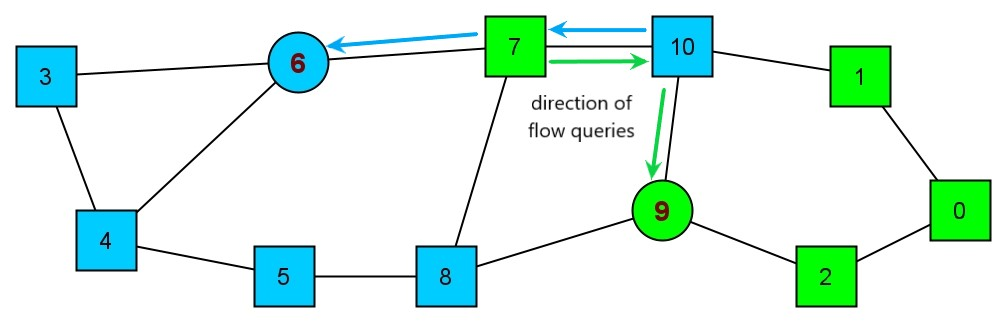
\includegraphics[width=0.85\textwidth]{Images/Abilene_overlap.jpg}
		\caption{Redundant traffic is generated for new flow queries of switches 7 and 10 to controllers 9 and 6 respectively, which can be avoided by swapping the clusters of the switches} \label{fig:overlap}
	\end{figure}
	
	\subsubsection{Search Space and Root State}
	The entire search space is a graph where each node corresponds to a \textit{state}. A state is a valid controller-switch assignment scheme where there are multiple controllers and every switch is assigned to a single controller. The \textit{Root state} of the graph is the resultant assignment of switches when LBC and CSA are applied on a network.
	
	\subsubsection{Child State}
	All the children of any node of the search space graph must be valid \textit{states}. Any \textit{Child state} is similar to its parent state except one switch, which is at the border of any cluster and is reassigned to the controller of the adjacent cluster. All such combinations constitute the set of Child states of any parent state.
	
	\subsubsection{Error Function}
	The error function $\varepsilon$ determines the acceptability of the current \textit{state} and is calculated as follows:
	\begin{equation}
	\varepsilon(state) = \sum_{i=1}^{k}\Bigg[\Big(L_i - \frac{L_{net}}{k}\Big)^2\Bigg]
	\end{equation}
	\begin{equation} \label{eqn:cload}
	L_i = \sum_{s\in S_i}l_{s}
	\end{equation}
	
	where, $L_i$ is the load of the $i^{th}$ controller, which is the cumulative load of the switches assigned to it. Squaring the differences give more priority to controllers whose loads are more imbalanced compared to others.
	
	\begin{figure}
		\centering
		\begin{subfigure}{0.3\textwidth}
			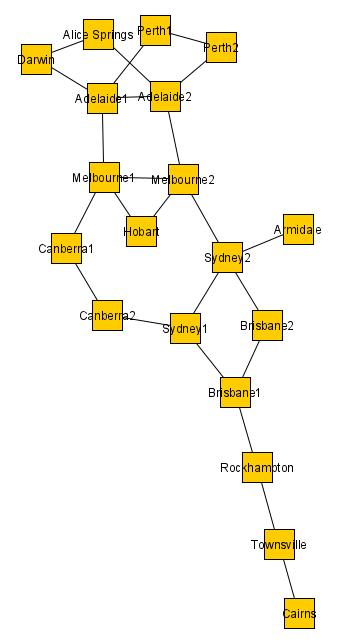
\includegraphics[width=\linewidth]{Images/Aarnet_Graph.jpg}
			\caption{Original Aarnet Network (rearranged)}
			\label{fig:aarnet2009}
		\end{subfigure}
		~
		\begin{subfigure}{0.3\textwidth}
			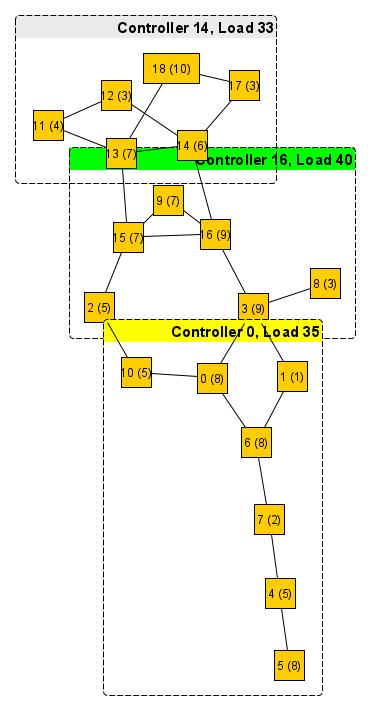
\includegraphics[width=\linewidth]{Images/Aarnet_Load_1.jpg}
			\caption{Root state with no child state}
			\label{fig:aarnet2009l1}
		\end{subfigure}
		~
		\begin{subfigure}{\textwidth}
			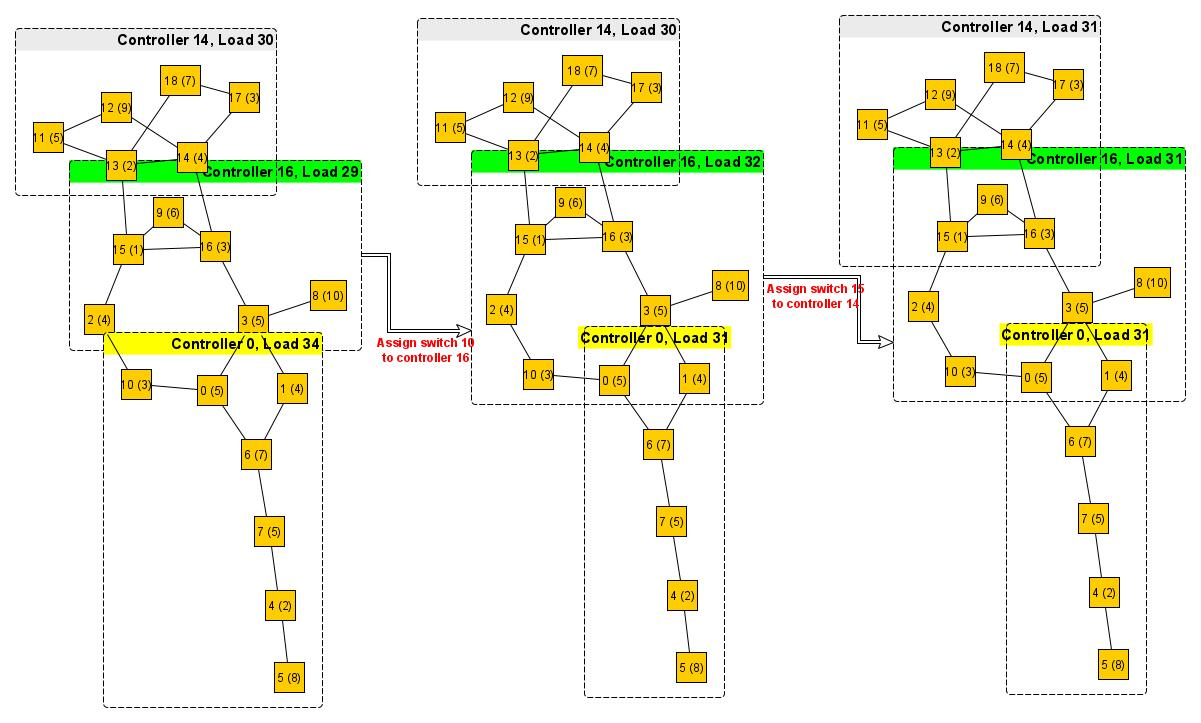
\includegraphics[width=\linewidth]{Images/Aarnet_Load_2.jpg}
			\caption{Optimal assignment scheme achieved after three iterations}
			\label{fig:aarnet2009l2}
		\end{subfigure}
		\caption{The BLB algorithm applied on Aarnet Network variations with randomized loads. Each switch is represented by a switch id, followed by its load. Each cluster has its own controller position and load marked above.}
	\end{figure}

	\subsubsection{Heuristic}
	A greedy heuristic is disadvantageous as it provides a sub-optimal solution. However, as my goal is not an absolute and optimal solution, rather a local optima where no clusters are overlapping, I select the error function as the heuristic. I use the Best First Search (BFS) technique with pruning to solve this problem, which selects the child state with the least error as the new assignment scheme in each iteration. When there is no child state with less error compared to the Root state (Figure \ref{fig:aarnet2009l1}), the child states are pruned to minimize computational complexity. Conversely, all the child states with equal or more error compared to the parent state are pruned at each iteration and the algorithm continues until the target state or a controller-switch assignment scheme with minimum error is achieved  (Figure \ref{fig:aarnet2009l2}). Extensive simulations suggest that the algorithm converges after a few iterations.
	
	
	\begin{algorithm}
		\SetAlgoLined
		\KwResult{Assignment of Switches, $S \rightarrow C$ }
		$S_{i=1}^k := $ \textbf{CSA} Clusters\;
		$state := S \rightarrow C$, current assignment of switches\;
		Set of all possible new states, $Pstates := \{state\}$\;
		\While{$Pstates \ne \emptyset$}{
			$state := \min\big(\varepsilon(Pstates)\big)$\;
			$Pstates := \emptyset$\;
			\ForEach{border switch $s\in S$}{
				New assignment $Nstate := state$\;
				Change assignment of switch $s$ to controller of adjacent cluster in $Nstate$\;
				\If{$\varepsilon(Nstate)<\varepsilon(state)$}{
					$Pstates := Pstates \cup \{Nstate\}$\;
				}
			}
		}
		\caption{BestFS Load Balancing (BLB)} \label{algo:blb}
	\end{algorithm}
	
	\section{Simulations} \label{simulations}
	
	The proposed mechanism clusters the network, places controllers, and performs load balancing on the clustered network. The following sections give a detailed description of the simulation environment and the performance metrics. In Section \ref{optimumK} optimum values for the decision variables $k$ and $\alpha$ are determined. Afterwards, in sections \ref{CPAnalysis} and \ref{LoadAnalysis}, my proposed algorithms are validated by comparing them with the state-of-the-art controller placement \cite{dbcp2017} and load balancing algorithms \cite{filali2018sdn}, respectively.
	
	\subsection{Simulation Environment}
	The simulation environment is developed using a high-level language C++, to perform experiments on existing networks topologies collected from the Internet Topology Zoo \cite{knight2011internet}. The Topology Zoo contains a total of 261 existing networks, out of which a few ($18$) have islands (isolated nodes). Therefore, I perform my experiments on the remaining networks. A summary of the experimental networks is given in Table \ref{tab:zooSummary}.
	\begin{table}
		\centering
		\caption{A summary of our Experimental Networks} \label{tab:zooSummary}
		\begin{tabular}{|l|c|}
			\hline
			\textbf{Category} & \textbf{Data} \\
			\hline
			Total number of networks & 243 \\
			\hline
			Number of unweighted networks & 134 \\
			\hline
			Maximum number of nodes & 754 \\
			\hline
			Minimum number of nodes & 4 \\
			\hline
			Networks with multi-edges & 82\\
			\hline
			Average Edge per Node & 1.285 \\
			\hline
		\end{tabular}
	\end{table}

	The weights of the links in the weighted networks are their bandwidths in \textit{Gb/s} (Giga-bits per second). These weights are converted into transmission latencies (milliseconds), assuming each control packet is 1500 bytes long. The maximum bandwidth is considered for links with variable bandwidths and all fiber-optic cables without available bandwidth information are assumed to have $1~Gb/s$ bandwidth. The networks with identical edge weights are considered as unweighted.
	
	I perform my load balancing simulations on the network with the highest number of nodes ($|S|=754$) to illustrate the performance of Best-first-search Load Balancing (BLB). The switches are assumed to have loads of 1000 to 5000 in terms of active flows per second, which is equivalent to the loads of data-center switches \cite{benson2010network}. I assume the network has $10$ controllers which are placed using LBC and CSA, and each controller has a maximum processing capacity of $1000K~flows/s$ which is adequate to support the maximum load of the networks in our simulations.
	\subsection{Performance Metrics}
	
	\begin{figure}
		\centering
		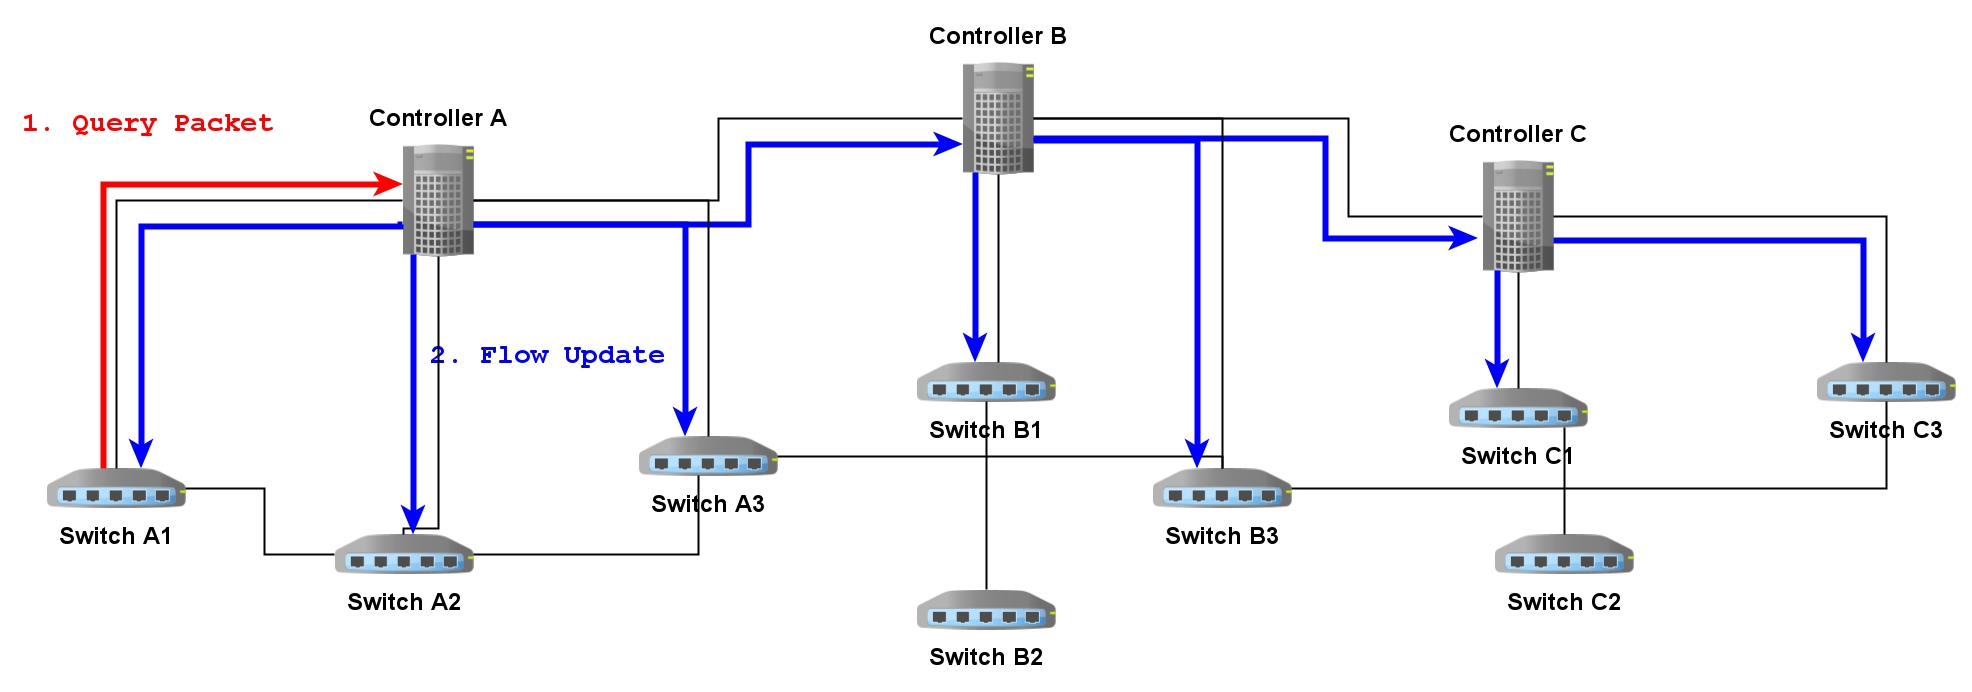
\includegraphics[width=\textwidth]{Images/new_flow.jpg}
		\caption{Setup of a new flow in the flow tables of the switches in the network} \label{new_flow}
	\end{figure}
	
	SDN switches match every incoming packet with appropriate flow tables. The result of a match can either be a \textit{hit} - which means the appropriate flow is already in a flow table, or, a \textit{miss} - in which case the flow is new and the switch asks its assigned controller for the next course of action. The assigned controller decides on a path for the flow and notifies the concerned switches to update their flow tables. However, for switches assigned to another controller, the corresponding controller is notified instead (Figure \ref{new_flow}). Therefore, the total time required to notify all the concerned switches about the new flow is the \textit{flow-setup latency}. I represent the average flow-setup latency ($\Omega_{avg}$) of the network as the average notification time of all possible pairs of switches in the network. For a network $S$ with $|S|$ number of switches, the average flow-setup latency can be calculated as follows:
	
	\begin{equation} \label{eqn:setupLatency}
	\Omega_{avg} = \frac{\sum_{s_i,s_d\in S} \{dis(s_i,c_i)+\max_{s_j\in path_{i,d}}\left(dis(c_i,c_j)+dis(c_j,s_j) \right) \}}{|S|\times |S-1|}
	\end{equation}
	
	here, $path_{i,d}$ is the shortest path from source $s_i$ to destination $s_d$, and $s_j$ is any switch in that path. The controllers of switches $s_i$ and $s_j$ are $c_i$ and $c_j$ respectively.
	
%	The processing latency of the controllers increase significantly for an imbalanced network, which can be calculated if the loads of the switches and controllers are known. Accordingly, the overall flow setup latency for a network $S$ can be calculated as follows:
%	\begin{equation}
%	\Delta(s_i) = \frac{\sum_{s_i,s_d\in S} \bigg[dis(s_i,c_i)+\max_{s_j\in path_{id}}\{dis(c_i,c_j)+dis(c_j,s_j) \} \bigg]}{|S|-1}
%	\end{equation}
%	\begin{equation}
%	\Omega(S) = \sum_{s_i\in S} \bigg[ \{\Delta(s_i)+\tau(c_i)\}\times l_{s_i} \bigg]
%	\end{equation}
	
%	here, $\Delta(s_i)$ is the average time required for a switch $s_i$ to add a new flow to its flow table in terms of transmission latency. The processing delay of its controller $c_i$ is denoted by $\tau(c_i)$ which can be calculated as explained in Section \ref{sysMod}, using the maximum processing capacity and load of the controller (Equation \ref{eqn:cload}). The average path-setup latency of the switch is the sum of its average transmission latency $\Delta(s_i)$, and the controller response time $\tau(c_i)$. Finally, the updated flow-setup latency of the network $\Omega(S)$, is the sum of the flow-setup latencies of all the switches, which can be calculated as the product of the average new-flow arrival rate ($l_{s_i}$) and the path-setup latency of the switches.
	
	\subsection{Decisive Variables} \label{optimumK}
	LBC clusters the network into $k$ sub-networks and CSA places a controller in each sub-network using the constant $\alpha$, which is a real number ranging from $0$ to $1$. The constant dictates the placement of controllers by controlling the priority of intra-cluster and inter-cluster distances. Applying LBC on a small network with varying values of $k$ and $\alpha$ (Figure \ref{fig:abileneA}) provide valuable insight on how the two variables affect the overall flow-setup latency of a network (Equation \ref{eqn:setupLatency}).
	
	\begin{figure}
		
		\centering
		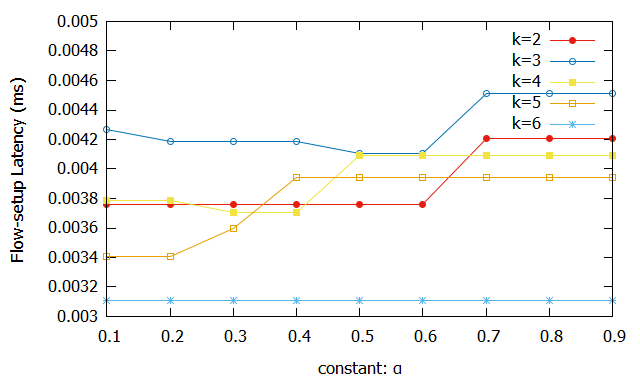
\includegraphics[width=0.9\textwidth]{Images/Abilene_Analysis.png}
		\caption{Average flow-setup latencies for varying values of $\alpha$ and $k$ in a network containing $|S|=11$ switches} \label{fig:abileneA}
		
	\end{figure}

	An increased number of clusters are formed when an excessively large amount of controllers are placed in a network. Consequently, the cluster-sizes are diminished, greatly reducing the number of viable controller positions in a specific cluster. Therefore, for a specific and large value of $k$, varying the value of $\alpha$ causes little or no change in placement and has no effect on overall flow-setup latency ($k=6$). For smaller values of $k$, the flow-setup latency gradually decreases and then increases ($k<5$). In some cases, the latency only increases as inter-controller distances increase ($k=5$), which indicates that no better placement is found for greater controller separation. The flow-setup latency is the lowest when $\alpha \ge 0.2$ and $\alpha \le 0.6$, which indicates that inter-controller communication contributes more in the flow-setup procedure when there are many controllers. However, in my experiments, I have used $\alpha=0.5$ to give equal priority to controller-to-switch and controller-to-controller communication.
	
	\begin{figure}
		\centering
		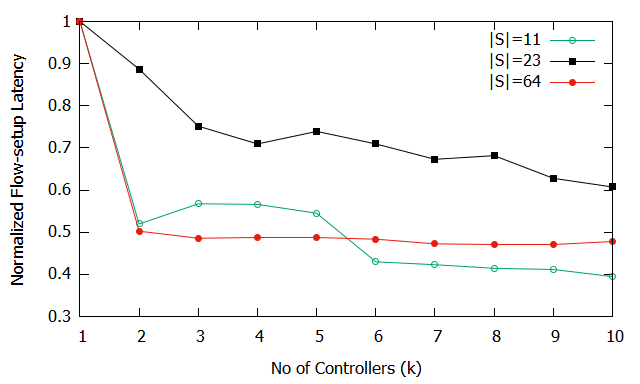
\includegraphics[width=0.9\textwidth]{Images/k_vs_l.png}
		\caption{Decreasing average flow-setup latencies with respect to number of controllers ($k$) for different networks. As the networks have varying latencies, they are normalized for comparison.} \label{fig:KvsL}
		\vspace{1cm}
		\centering
		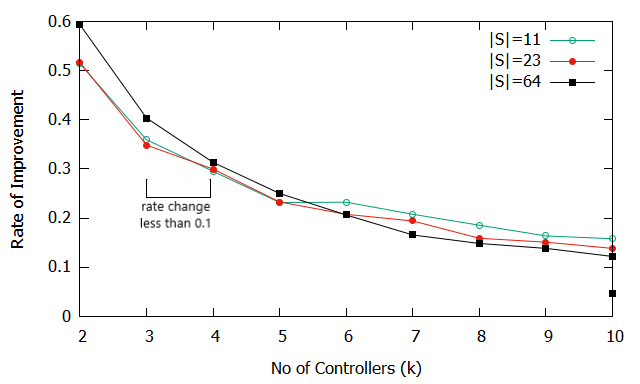
\includegraphics[width=0.9\textwidth]{Images/cutoff.png}
		\caption{Gradually decreasing improvement ratio with respect to number of controllers ($k$) for networks of different sizes} \label{fig:cutoff}
	\end{figure}

	The flow-setup latency of a network decreases as the number of controllers increase, with a few exceptions due to variations in network topology (Figure \ref{fig:KvsL}). The rate of decrease is greater for smaller networks compared to larger networks as controller/switch ratio increase drastically for smaller networks. Accordingly, the setup latency is minimum when $k$ is equal to the total number of nodes in a network, which however, invalidates one of the firsthand benefits of placing controllers (simplifying nodes and reducing costs). In order to determine the optimum number of controller $k$ for a network $S$, we define an improvement ratio:
	
	\begin{equation}
	improvement~ratio_k = \frac{Latency_1}{Latency_k\times k}
	\end{equation}
	
	here, $Latency_1$ and $Latency_k$ are the flow-setup latencies when the number of controllers are 1 and $k$ respectively.
	
	The improvement ratio for a network decreases gradually with respect to increasing number of controllers (Figure \ref{fig:cutoff}). I observe that the improvement rate \textit{change} decreases drastically to less than $0.1$ from more than $0.2$ and $0.15$, after adding 4 controllers to the network where $|S|=64$ and 3 controllers to the other two networks, respectively. Therefore, I cease adding controllers when the improvement rate change drops below $0.1$. Consequently, the resultant average switch/controller ratio of the 238 networks is $12.79$. According to expert opinions \cite{cpp2012heller}, a network with $34$ nodes requires approximately $3$ controllers to function efficiently and one more to handle failures, which supports our optimal $k$ derivation in terms of average switch/controller ratio.
	
	\subsection{Controller Placement} \label{CPAnalysis}
	In this section I evaluate my static controller placement method (LBC+CSA) by comparing it to the well-known algorithm DBCP \cite{dbcp2017} and the algorithm DBC \cite{aziz2019degree}. DBCP places controllers based on the density of nodes and the minimum distance to higher density nodes. In order to compare the algorithms, I simulate both DBC and LBC with the same number of controllers as DBCP when clustering the networks from the Zoo Topology. DBCP underperforms compared to LBC and DBC when the network has high connectivity (e.g. star topology) or when all nodes have equal density (e.g. ring topology). My simulations using the remaining networks suggest that LBC+CSA outperforms both DBCP and DBC in terms of flow-setup latencies.
	
	The flow-setup latency results of the simulations vary greatly for different networks. Therefore, I represent the latencies of DBCP and DBC as a ratio of the latencies of LBC+CSA and plot their averages for a given range of network sizes (Figure \ref{fig:Fcomparison}). The average latency of all the networks with network sizes less than $10$ are plotted for $|S|=5$, those greater than 9 and less than 20 are plotted for $|S|=15$, and so on. Although DBC performs better for certain unweighted networks, LBC+CSA outperforms both DBCP and DBC in 78\% and 72\% of the simulated networks, respectively.
	
	\begin{figure}
		\centering
		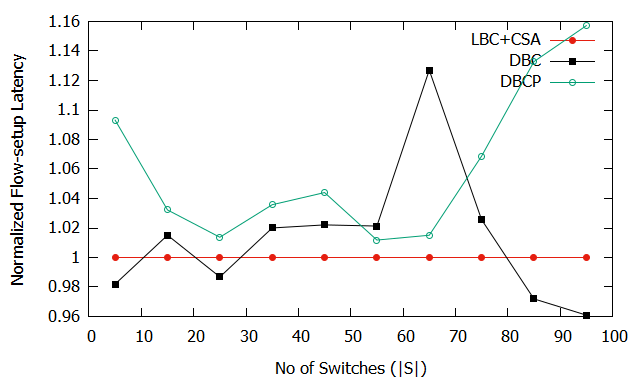
\includegraphics[width=0.9\textwidth]{Images/forced_comparison.png}
		\caption{Comparison among LBC+CSA, DBCP and DBC, in terms of normalized flow-setup latency} \label{fig:Fcomparison}
	\end{figure}
	
	\subsection{Load Balancing} \label{LoadAnalysis}
	BLB balances the loads of the controllers by swapping clusters of border nodes to avoid overlapping cluster formations. I set the maximum iteration limit of BLB to $100$ and compare with the algorithm MSDA \cite{filali2018sdn, fragiadakis2016strategyproof} in terms of maximum load imbalance. The loads of the switches are randomly assigned within the range $1000$ to $5000$ with equal probability. Therefore, the average switch load is $2500 flows/s$ and the target controller load is $188.5K flows/s$ (Figure \ref{fig:Lcomparison}). The global precedence list of MSDA is calculated by multiplying transmission latency with average sojourn time or controller processing time. However, transmission latencies are usually greater than processing latencies, which results in load imbalance. Furthermore, when the maximum controller capacity is decreased substantially, MSDA underperforms as the preferences of the controllers and switches cannot be satisfied. The simulation suggests that BLB outperforms MSDA in terms of controller load, specially for controllers 8 and 9 (Figure \ref{fig:Lcomparison}). The maximum iteration limit can be increased for better accuracy and performance.
	
	\begin{figure}
		\centering
		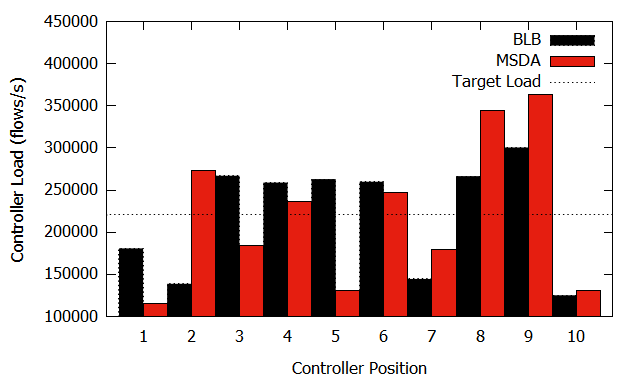
\includegraphics[width=0.9\textwidth]{Images/load_comparison.png}
		\caption{Comparison between BLB and MSDA in terms of load per controller} \label{fig:Lcomparison}
		\vspace{1cm}
		\centering
		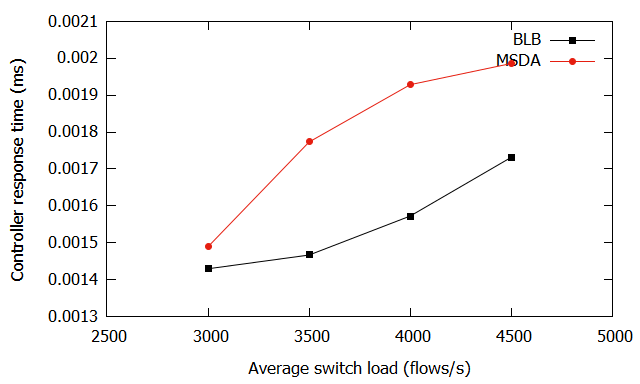
\includegraphics[width=0.9\textwidth]{Images/response_comparison.png}
		\caption{Gradually decreasing average response times for varying switch loads} \label{fig:Rcomparison}
	\end{figure}
	
	
	The Figure \ref{fig:Rcomparison} represents the comparison between BLB and MSDA in terms of maximum controller response times for different average switch loads. The response times increase with increasing switch loads as the controller loads also increase significantly. The comparison shows that BLB outperforms MSDA in terms of average controller response times. The average controller response time is reduced by an average of $13\%$.

	\section{Conclusion} \label{conclusion}
	In this paper, I propose a novel controller assignment method which clusters the network, places controllers and balanced loads to reduce overall flow-setup latency of the network. My proposed method address the Controller Placement Problem (CPP) and outperforms several state-of-the-art algorithms based on various performance metrics. My proposed method has many advantages over other algorithms which include -- having polynomial time complexity, providing an optimal number of clusters, decreasing controller response time and flow-setup latency simultaneously. My proposed algorithm BLB can be extended to work on any network and to optimize any parameter by improving and introducing different error functions. Future work can include variable controller capacities when balancing controller loads. My proposed method can also be extended to facilitate simultaneous optimization of multiple network parameters, which can be very helpful to network operators.
	
	\bibliographystyle{elsarticle-num} 
	\bibliography{mybib}
\end{document}